Em auxílio à prova do Teorema \ref{teo:trans}, vamos discutir propriedades 
de monotonicidade da função $\tep$.  Para isto, construiremos um
modelo probabilístico em que 
os modelos de percolação com os
diversos valores de $p$ possíveis estão acoplados.
Esta construção, a que chamaremos de {\em modelo padrão},  
será útil também em outros casos.

Seja ${\cal Z}:=\{Z_e, e\in\ed\}$ uma 
família de
v.a.'s i.i.d. com distribuição
comum uniforme em $[0,1]$. $\pp$ denotará a probabilidade neste modelo.

Um elo $e$ da rede será dito {\em $p$-aberto} se $$Z_e<p$$ e {\em $p$-fechado} caso
contrário. Podemos então construir o modelo de percolação
com parâmetro $p$ usando elos $p$-abertos e $p$-fechados deste modelo, 
da mesma forma como na seção anterior.

\vs

\blem
\label{lem:tep}
$\tep$ é não-decrescente em $p$.
\elem

\vs

\noindent{\bf Prova}

Seja $C_p$ o aglomerado da origem no modelo acima
(com a conectividade através de elos $p$-abertos). Temos que $$\tep=\pp(|C_p|=\infty).$$
Por outro lado, $$C_p\subset C_{p'}$$ quando $p<p'$, pois neste caso 
um elo $p$-aberto está necessariamente $p'$-aberto.
Concluimos que $$\tep=\pp(|C_p|=\infty)\leq\pp(|C_{p'}|=\infty)=\tepl.\bo$$

\vs

Para o próximo resultado, monotonicidade na dimensão, notemos que podemos construir 
o modelo de percolação em $d$ dimensões num hiperplano $d$-dimensional da rede 
$d+1$-dimensional contendo a origem, declarando fechados os elos ligando o 
hiperplano ao restante do espaço e usando ${\cal X}$ para os demais elos. 
Denotando por $\tilde C$ o aglomerado da origem neste modelo, temos claramente que
$\tilde C\subset C$ e logo $$\tep:=\ted=\pdu(|\tilde C|=\infty)\leq
\pdu(|C|=\infty)=\tedu.$$ Isto prova o seguinte.   

\vs

\blem
\label{lem:ted}
$\ted$ é não-decrescente em $d$.
\elem

\vs

Pelos dois lemas acima, torna-se suficiente, para provarmos o Teorema \ref{teo:trans},
mostrarmos os seguintes resultados.

\bprop
\label{prop:trans1}
Para $d\geq2$ e $p$ suficientemente próximo de $0$ $$\tep=0.$$
\eprop

\bprop
\label{prop:trans2}
Para $d=2$ e $p$ suficientemente próximo de $1$ $$\tep>0.$$
\eprop

Como veremos nas demonstrações destes resultados, abaixo, é suficiente no
primeiro tomarmos $p<1/{(2d-1)}$ e no segundo $p>2/3$.

\vs

\noindent{\bf Prova da Proposição \ref{prop:trans1}} 

É suficiente mostrar que $\xip:=\ep\cl<\infty$ para $p$ próximo de 0.

Podemos escrever $$\cl=\sum_{x\in\zzd}\ind_{\{0\lr x\}},$$ onde $\ind_{\{\cdot\}}$ é a
função indicadora, isto é, 
$$\ind_A(\om)=\cases{1,& se $\om\in A$\cr 
                    0,& caso contrário,}$$
e logo
\beq
\label{eq:quip}
\xip=\sum_{x\in\zzd}\p(0\lr x).
\eeq
Podemos reescrever a probabilidade acima como
$\p(\cup_{\ga}\{\ga\mbox{ está aberto}\}),$
onde a união é sobre caminhos conectando $0$ a $x$.
Temos então de~(\ref{eq:quip}) e a subaditividade que
$$\xip\leq\sum_{x\in\zzd}\sum_{\ga}\p(\ga\, \mbox{está aberto}),$$
onde a segunda soma é sobre os caminhos $\ga$ conectando $0$ a $x$.
A dupla soma pode ser então reordenada em 
$$\sum_{n\geq0}\sum_{|\ga|=n}\p(\ga\, \mbox{está aberto}),$$
onde a segunda soma é sobre os caminhos $\ga$ partindo da origem
e de comprimento $n$ (isto é, caminhos $\ga=\{e_1,\ldots,e_n\}$
em que $x_1=0$). A probabilidade acima vale $p^n$ independentemente de $\ga$.
Portanto temos que 
\beq\label{eq:trans1}\xip=\sum_{n\geq0}\sigma(n)p^n,\eeq
onde $\sigma(n)$ denota
o número de caminhos partindo da origem e de comprimento $n$.

Um argumento combinatório simples revela que, para $n\geq1$, 
$$\sigma(n)\leq 2d(2d-1)^{n-1}.$$
De fato, o primeiro passo do caminho tem $2d$ possíveis sítios de destino, 
enquanto que
a partir do segundo até o final, cada passo tem {\em no máximo} $2d-1$ possíveis
sítios de destino (devido à ausência de {\em loops}). Temos
$$\xip\leq\sum_{n\geq1}2dp[(2d-1)p]^{n-1}+1$$
e para a série ser convergente, basta termos $p<1/{(2d-1)}.\bo$

\vs

\noindent{\bf Prova da Proposição \ref{prop:trans2}}
\label{trans2}
Consideremos a rede bidimensional dual de $\zt$, $$\zs=\zt+(1/2,1/2).$$
$\zs$ é um deslocamento de $\zt$ por $1/2$ unidade em cada direção coordenada.
Volumes finitos superpostos de $\zt$ e $\zs$ são ilustrados abaixo, o de $\zt$
em linhas cheias, linhas tracejadas para $\zs$.

\vs

\bec

%\input du1
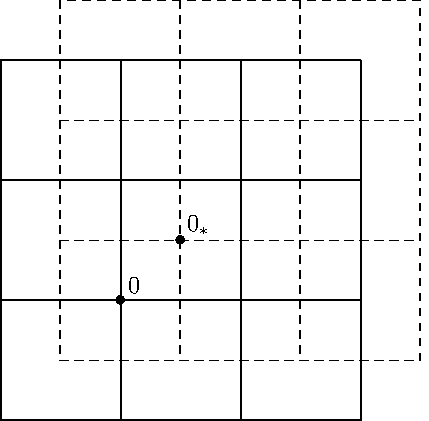
\includegraphics{du1}

\eec

\vs

Notemos que há uma relação 1 a 1 entre os sítios e elos de $\zt$ e aqueles
de $\zs$. Seja a relação (1 a 1) $e\to\es$ entre elos de $\zt$ e $\zs$ que associa 
a cada elo da primeira rede o elo secante da rede dual, como na figura a
seguir.

\bec
%\input sec.tex
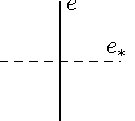
\includegraphics{sec}
\eec

Definiremos um modelo de percolação em $\zs$ induzido pelo modelo em $\zt$
declarando $\es$ aberto ou fechado conforme $e$ esteja aberto ou fechado,
respectivamente.

No que se segue, um {\em circuito} será um caminho $\{e_1,e_2,\ldots,e_n\}$
tal que $y_n=x_1$, isto é, um caminho que se fecha sobre si mesmo.

A ocorrência de um aglomerado da origem finito em $\zt$ está associada à
existência de um circuito fechado (isto é, um circuito de elos fechados) na
rede dual ao redor da origem. Isto se deve ao fato de que se o aglomerado da
origem for finito, os elos da fronteira do aglomerado (isto é, elos ligando
sítios do aglomerado a sítios fora do aglomerado), obviamente fechados, estão
sempre dispostos de tal forma que os elos correspondentes do dual formam um 
circuito, que será então fechado. A figura a seguir ilustra este fato geométrico
elementar, bastante
intuitivo (o aglomerado da origem aparece em linhas cheias, sua fronteira em linhas
pontilhadas e o circuito no dual em linhas tracejadas) e, como a
prova é longa e tediosa (vide \cite{kn:K2} página 386 e
a Proposição~\ref{pro:geo} na página~\pageref{pro:geo} destas notas), 
não a apresentaremos neste texto.

\vs

\bec

%\input cir.tex
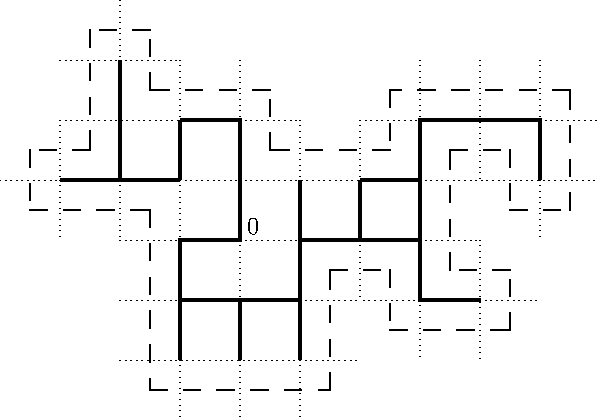
\includegraphics{cir}

\eec

\vs

Seguimos com a demonstração da Proposição \ref{prop:trans2}.

Vamos mostrar que a probabilidade de o aglomerado da origem ser finito
é estritamente menor do que 1 para $p$ suficientemente próximo de 1. Para
isto, em vista do fato geométrico acima, bastará argumentar que a probabilidade
de haver algum circuito fechado na rede dual ao redor da origem é estritamente
menor do que 1 para $p$ suficientemente próximo de 1. O argumento é semelhante
ao {\em argumento de Peierls} para demonstrar a ocorrência de magnetização no
modelo de Ising.
\beqnn
\p(\mbox{há um circuito fechado na rede dual ao redor da origem})\\
\leq\sum_{\ga}\p(\ga\,\mbox{está fechado}),
\quad\quad\quad\quad\quad\quad\quad\quad\quad
\eeqnn 
onde a soma é sobre todos os circuitos $\ga$ ao redor da origem. Ela pode ser
reordenada da seguinte maneira
$$
\sum_{n\geq4}\sum_{|\ga|=n}\p(\ga\,\mbox{está fechado}),
$$
onde a segunda soma é sobre circuitos $\ga$ ao redor da origem de comprimento $n$.

Está claro que a probabilidade no interior das somas depende apenas de $n$ e vale
$(1-p)^n$. Portanto, a expressão acima fica
$$
\sum_{n\geq4}\ln(1-p)^n,
$$
onde $\ln$ denota o número de circuitos na rede dual ao redor da origem de 
comprimento $n$.

O seguinte argumento produz uma cota superior útil para $\ln$. Qualquer circuito
de comprimento $n$ da rede dual ao redor da origem deve cruzar um elo da rede
original da forma $((0,k),(0,k+1))$, para algum $-n/2\leq k\leq n/2$. A partir deste
elo secante, cada um dos $n-1$ elos subseqüentes pode ser colocado de no máximo 
$3$ maneiras diferentes. Por isto
$$\ln\leq n3^{n-1}.$$
Substituindo na soma acima, temos
$$
\sum_{n\geq4}\frac{n}{3}[3(1-p)]^n,
$$
que é uma função contínua e decrescente em $p$ quando $p>2/3$, anulando-se 
quando $p=1$. Segue-se que existe $p_0<1$ tal que a expressão acima é
estritamente menor do que 1 para $p>p_0$.$\bo$

\vs

Uma melhoria do argumento acima que mostra que a probabilidade de o aglomerado
da origem ser infinito ($\tep$) é
estritamente positiva para $p>2/3$ é o seguinte.
   
Denotemos por $Q_M$ o quadrado centrado na origem e de lado $2M+1$.
Seja $A_M$ o evento que todos os elos de $Q_M$ estejam abertos e
$B_M$ o evento de haver um circuito fechado na rede dual {\em completamente
fora de} $Q_M$.

Repetindo o argumento da demonstração acima, temos
$$
\p(B_M)\leq\sum_{n\geq 8M+4}\frac{n}{3}[3(1-p)]^n.  
$$
Dado $p>2/3$, esta expressão pode ser tornada estritamente menor do que 1 
escolhendo-se $M$ suficientemente grande, digamos $M_0$. Portanto
\beq\label{eq:pei}\p(B_{M_0}^c)>0.\eeq

Agora, na intersecção dos eventos $A_{M_0}$ e $B_{M_0}^c$, o aglomerado da origem é
infinito. Além disso, $A_{M_0}$ e $B_{M_0}^c$ são independentes, pois dependem de
conjuntos disjuntos de elos. Logo, de (\ref{eq:pei}) concluimos que
$$
\tep\geq\p(A_{M_0}\cap B_{M_0}^c)=\p(A_{M_0})\p(B_{M_0}^c)>0,
$$
pois $\p(A_{M_0})>0$ (ainda que próximo de 0). O argumento está completo. 

\vs

A probabilidade crítica $\pce$ depende da dimensão e podemos denotá-la
$\pce(d)$. As proposições acima mostram que 
$$\frac{1}{2d-1}\leq\pce(d)\leq\frac{2}{3}.$$ Kesten~\cite{kn:K3} mostrou que
$$\pce(d)\sim\frac{1}{2d}$$ para dimensões grandes.

\vs

O Teorema~\ref{teo:trans} não diz nada sobre o que acontece em $p=\pce$.
Como veremos no Capítulo~4, $\tep$ é uma função contínua, exceto possivelmente
em $p=\pce$. Se $\tepc=0$, então $\tep$ será contínua e seu gráfico se
parecerá com o da figura à esquerda a seguir.
Caso contrário, o gráfico será mais parecido com o da figura à direita.

\vs
%\input cont
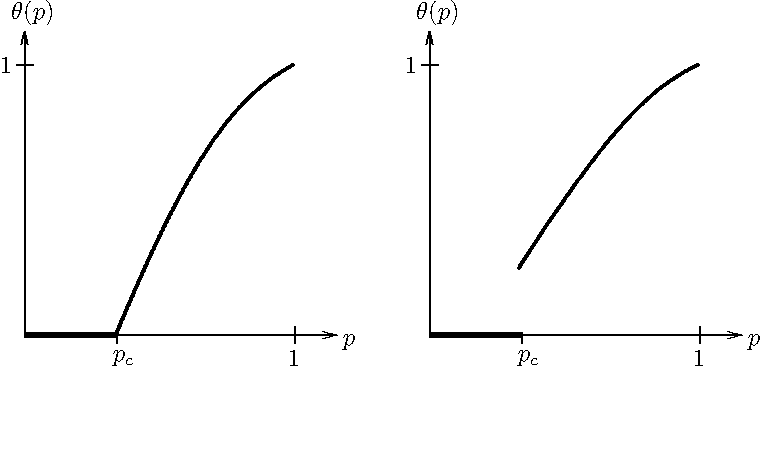
\includegraphics{cont}

Qual caso vale é uma questão em aberto para $d$ genérico, mas se acredita que $\tep$ seja
contínua. Isto está de fato provado em 2 dimensões e em dimensões grandes.
Veremos o caso bidimensional no Capítulo~5 e discutiremos um método de
ataque ao problema em mais dimensões no Capítulo~6.


